%++++++++++++++++++++++++++++++++++++++++
% Don't modify this section unless you know what you're doing!
\documentclass[letterpaper,12pt]{article}
\usepackage{tabularx} % extra features for tabular environment
\usepackage{amsmath}  % improve math presentation
\usepackage{graphicx} % takes care of graphic including machinery
\usepackage[margin=0.75in,letterpaper]{geometry} % decreases margins
\usepackage{cite} % takes care of citations
\usepackage[final]{hyperref} % adds hyper links inside the generated pdf file
\usepackage{listings}
\usepackage{csvsimple}
\usepackage{verbatim}
\usepackage{graphicx} % Allows including images
\hypersetup{
	colorlinks=true,       % false: boxed links; true: colored links
	linkcolor=blue,        % color of internal links
	citecolor=blue,        % color of links to bibliography
	filecolor=magenta,     % color of file links
	urlcolor=blue         
}
%++++++++++++++++++++++++++++++++++++++++
\begin{document}
\title{PyLab - Ohm and Power laws}
\author{Fredrik Dahl Bråten, Pankaj Patil}
\date{\today}
\maketitle

\section{Exercise 1:  Introduction to fitting methods}

\subsection{Introduction}

In this exercise, we fit the experimental data to a linear function.  

\subsection{Methods}

We followed the method descibed in the lab manual to setup the circuit. Following steps were 
performed,

\begin{enumerate}
  \item Connect the ameter, voltmeter, and power supply to the resistor. The setup of the circuit is shown (Figure 1).
  \item Vary the voltage on the power supply.
  \item Record the voltage and current from the multimeters, along with uncertainty.
  \item Change the voltage, and record the new values. This step was repeated to record more data  points.
  \item Observations were recorded in csv files, separate file for 100 kiloohm and Potentiometer.
  \item After performing all the above measurements, disconnected the power, and switch the voltmeter to resistance. The resistance value was noted for reference.
\end{enumerate}

\begin{center}
  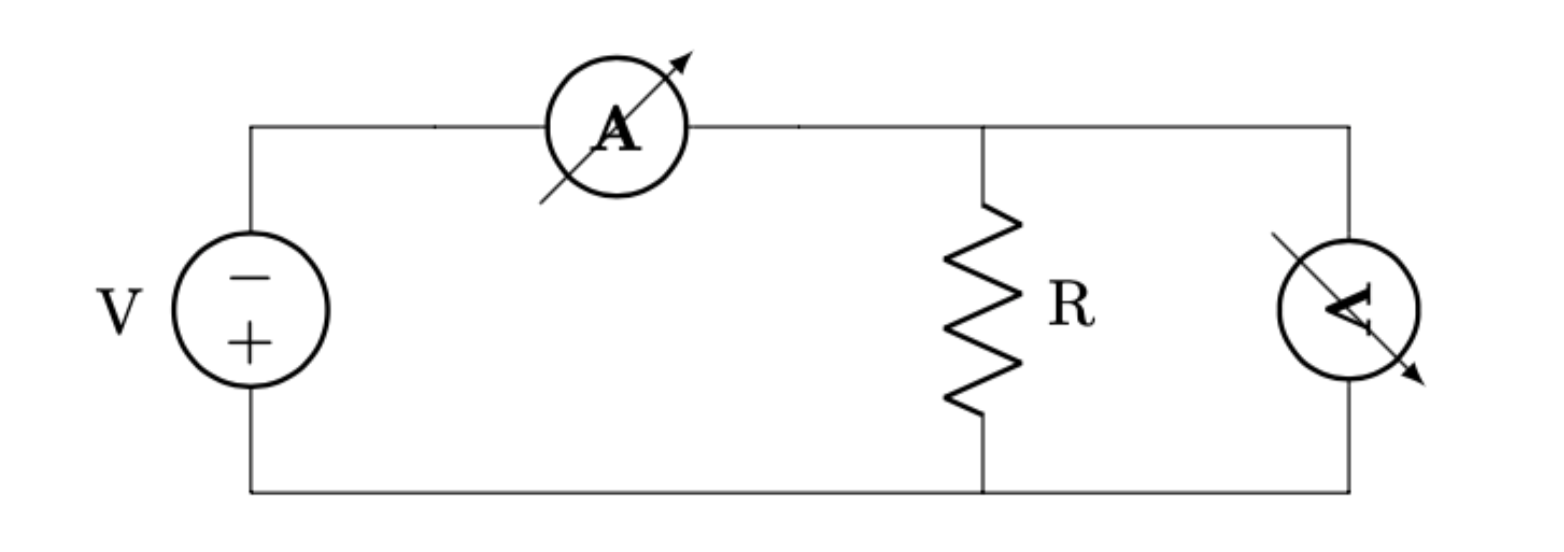
\includegraphics[width=1.0\linewidth]{../lab_1_ex_1_setup.png}    
\end{center}
Folowing observations were made for the instruments,

\begin{enumerate}
  \item One of the multimeter was faulty, and we discarded the readings takes from that multimeter.
  \item We accidently changed the potentiometer value, so we had to repeat the set of observations for it.
\end{enumerate}

\csvautotabular{../100k.csv}
\linebreak
\csvautotabular{../Potentiometer.csv}

\subsection{Results}
\subsection{Analysis \& Discussion }

\begin{center}
    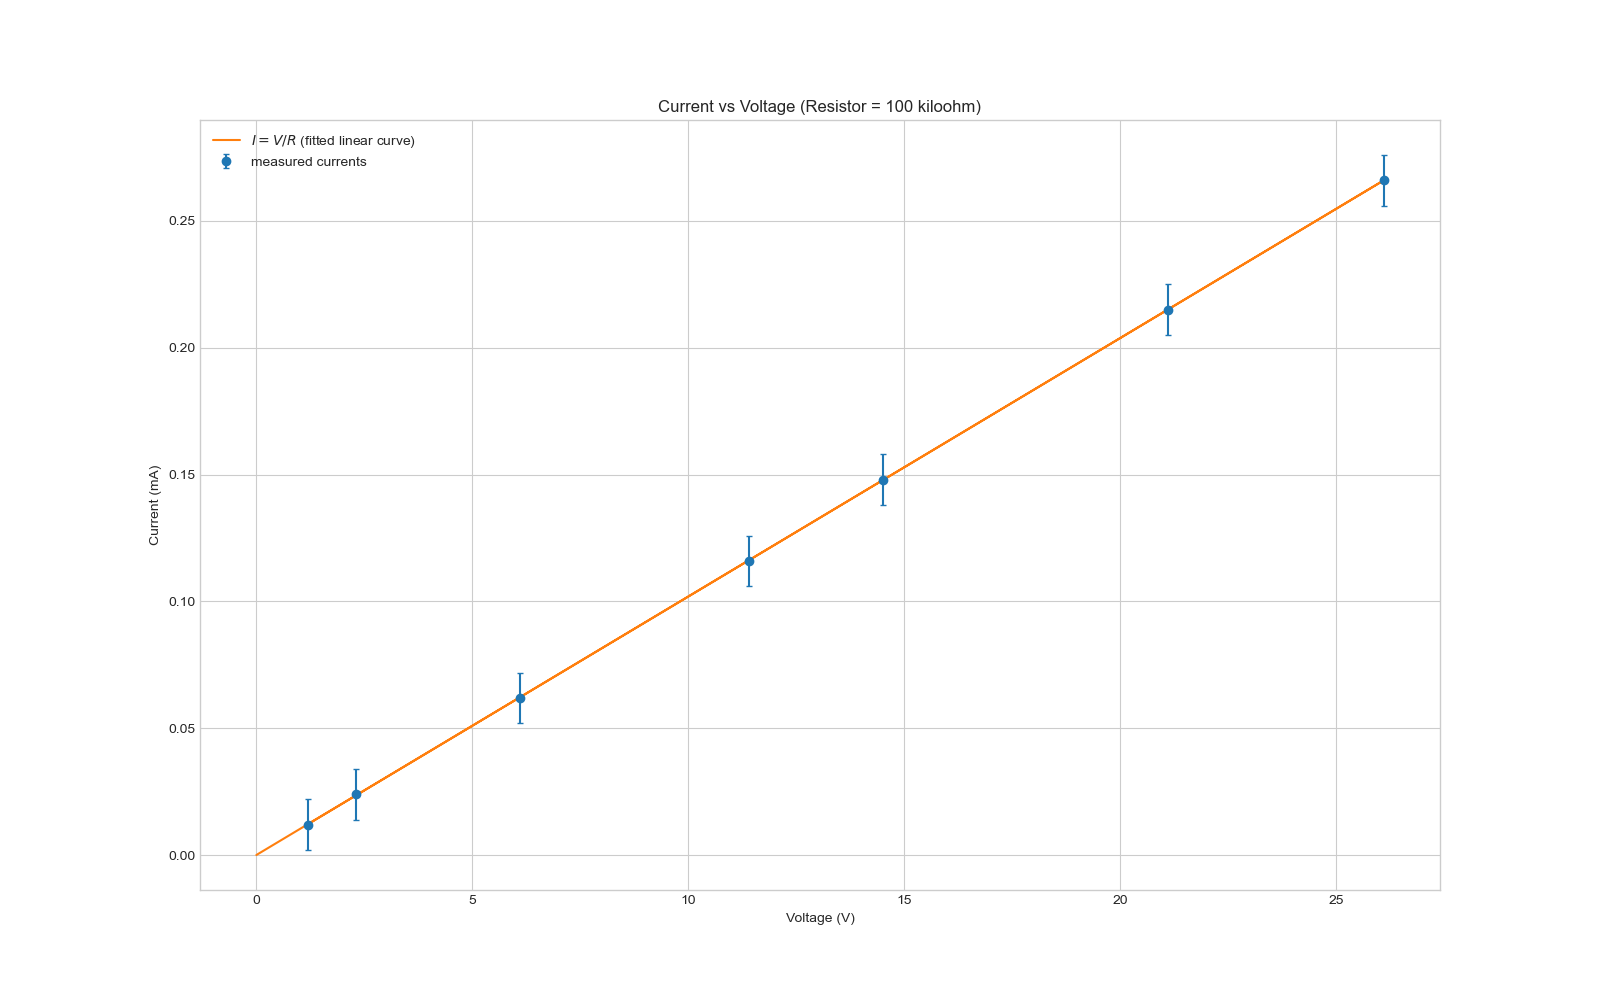
\includegraphics[width=1.0\linewidth]{../lab_1_ex_1_plot_100k.png}    
    \includegraphics[width=1.0\linewidth]{../lab_1_ex_1_plot_potentiometer.png}    
\end{center}

\subsection{Conclusions}

\pagebreak

\section{Exercise 3:  Nonlinear fitting methods II}

\subsection{Introduction}

\csvautotabular{../100k.csv}
\linebreak
\csvautotabular{../Potentiometer.csv}
\subsection{Methods}
\subsection{Results}
\subsection{Analysis \& Discussion }

\begin{center}
    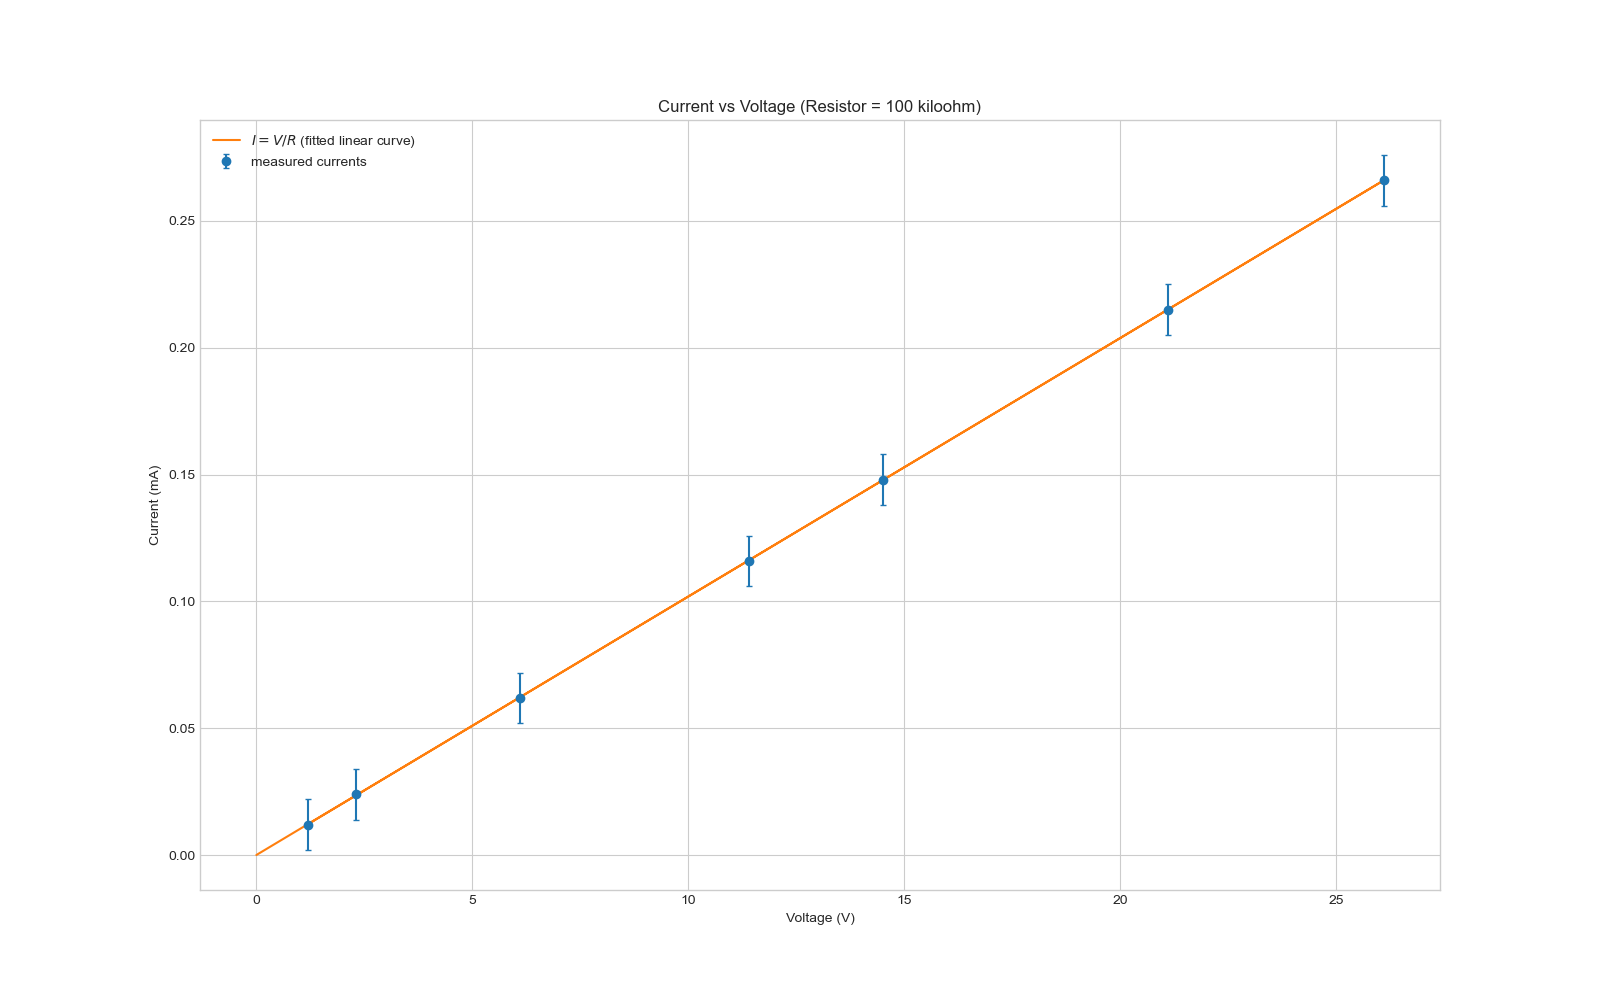
\includegraphics[width=1.0\linewidth]{../lab_1_ex_1_plot_100k.png}    
    \includegraphics[width=1.0\linewidth]{../lab_1_ex_1_plot_potentiometer.png}    
\end{center}

\subsection{Conclusions}

\pagebreak

\begin{center}
  \section*{Appendix}
\end{center}

\subsection*{Python Code: Exercise 1}

\verbatiminput{../lab_1_ex_1_code.py}

\pagebreak

\subsection*{Python Code: Exercise 3}

\verbatiminput{../lab_1_ex_1_code.py}

\pagebreak

\begin{thebibliography}{99}

\bibitem{melissinos}

\end{thebibliography}

\end{document}
